\subsection{Transformer:}

Calculate the Voltage ( $V_{0}$ ) in $R_{L}$ given the following resistors:

\begin{figure}[H]
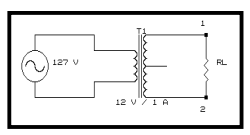
\includegraphics[scale=1]{transformer.png}
\centering \linebreak \linebreak Figure 5.1.0: Transformer.
\end{figure}

For: $R_{L} = 100\Omega$ and $R_{L} = 22\Omega$.

\begin{itemize}
\item {\bfseries\itshape Where the voltage at the output of the transformer is:
\begin{tasks}
\task $V_{T}$ = 12 V
\end{tasks}} \hfill
\end{itemize}

{\bfseries\itshape\color{Maroon}{Solution:}} \hfill \break

\begin{itemize}
\item {\bfseries\itshape\color{Violet}{For $R_{L} = 100\Omega$:}} \hfill \break
{\bfseries\itshape\color{Brown}{
\begin{tasks}
\task Using Ohm's Law: $V$ = $(\ I\ )(\ R\ )$. \hfill \break
\end{tasks}}}

\end{itemize}

\begin{ceqn}
\begin{align}
V_{0} = ( 100\Omega )( I_{0} )
\end{align}
\end{ceqn} \hfill

\begin{itemize}
\item {\bfseries\itshape\color{Violet}{For $I_{0}$:}} \hfill \break
\end{itemize}

\begin{ceqn}
\begin{align}
I_{0} = \frac{12V}{100\Omega} = 0.12 A
\end{align}
\end{ceqn} \hfill

\begin{itemize}
\item {\bfseries\itshape\color{Violet}{Substituting ( 19 ) in ( 18 ):}} \hfill \break
\end{itemize}

\begin{ceqn}
\begin{align}
V_{0} &= ( 100\Omega )( 0.12A ) \\
&= 12 V 
\end{align}
\end{ceqn} \hfill

\pagebreak

\begin{itemize}
\item {\bfseries\itshape\color{Violet}{For $R_{L} = 22\Omega$:}} \hfill \break
{\bfseries\itshape\color{Brown}{
\begin{tasks}
\task Using Ohm's Law: $V$ = $(\ I\ )(\ R\ )$. \hfill \break
\end{tasks}}}
\end{itemize}

\begin{ceqn}
\begin{align}
V_{0} = ( 22\Omega )( I_{0} )
\end{align}
\end{ceqn} \hfill

\begin{itemize}
\item {\bfseries\itshape\color{Violet}{For $I_{0}$:}} \hfill \break
\end{itemize}

\begin{ceqn}
\begin{align}
I_{0} = \frac{12V}{22\Omega} = 0.54 A
\end{align}
\end{ceqn} \hfill

\begin{itemize}
\item {\bfseries\itshape\color{Violet}{Substituting ( 23 ) in ( 22 ):}} \hfill \break
\end{itemize}

\begin{ceqn}
\begin{align}
V_{0} &= ( 22\Omega )( 0.54A ) \\
&= 11.8 V 
\end{align}
\end{ceqn} \hfill

\pagebreak